

\tikzset{every picture/.style={line width=1.2pt}} %set default line width to 0.75pt        

\begin{tikzpicture}[x=1.3pt,y=1.3pt,yscale=-1,xscale=1]

%Curve Lines [id:da7541991933684267] 
\draw [color={rgb, 255:red, 0; green, 0; blue, 0 }  ,draw opacity=1 ]   (189.71,139.79) .. controls (217.57,219.97) and (240.15,251.07) .. (319.89,260.89) ;
%Shape: Axis 2D [id:dp9714753284680302] 
\draw [color={rgb, 255:red, 0; green, 0; blue, 0 }  ,draw opacity=0.85 ] (155.98,276.54) -- (343.18,276.54)(174.7,122.41) -- (174.7,293.67) (336.18,271.54) -- (343.18,276.54) -- (336.18,281.54) (169.7,129.41) -- (174.7,122.41) -- (179.7,129.41)  ;
%Straight Lines [id:da48280757585710066] 
\draw [color={rgb, 255:red, 0; green, 0; blue, 0 }  ,draw opacity=1 ]   (189.71,139.79) -- (190.21,260.14) ;
%Straight Lines [id:da9906712361639143] 
\draw [color={rgb, 255:red, 0; green, 0; blue, 0 }  ,draw opacity=1 ]   (319.89,260.89) -- (190.21,260.14) ;
%Straight Lines [id:da08991361869671644] 
\draw  [dash pattern={on 0.84pt off 2.51pt}]  (239.95,231.25) -- (240.04,276.86) ;
%Straight Lines [id:da30586417052351544] 
\draw  [dash pattern={on 0.84pt off 2.51pt}]  (239.95,231.25) -- (174.75,231.42) ;

% Text Node
\draw (239.52,203.55) node [anchor=north west][inner sep=0.75pt]  [font=\scriptsize,color={rgb, 255:red, 0; green, 0; blue, 0 }  ,opacity=1 ,xscale=2,yscale=2]  {$dk=x$};
% Text Node
\draw (170.33,106.57) node [anchor=north west][inner sep=0.75pt]  [font=\scriptsize,xscale=2,yscale=2]  {$k$};
% Text Node
\draw (346,269.07) node [anchor=north west][inner sep=0.75pt]  [font=\scriptsize,xscale=2,yscale=2]  {$d$};
% Text Node
\draw (185.5,279.65) node [anchor=north west][inner sep=0.75pt]  [font=\scriptsize,xscale=2,yscale=2]  {$1$};
% Text Node
\draw (236.25,277.9) node [anchor=north west][inner sep=0.75pt]  [font=\scriptsize,xscale=2,yscale=2]  {$y$};
% Text Node
\draw (159.75,218.4) node [anchor=north west][inner sep=0.75pt]  [font=\scriptsize,xscale=2,yscale=2]  {$\dfrac{x}{y}$};
% Text Node
\draw (164.25,134.57) node [anchor=north west][inner sep=0.75pt]  [font=\scriptsize,xscale=2,yscale=2]  {$x$};
% Text Node
\draw (316.33,277.82) node [anchor=north west][inner sep=0.75pt]  [font=\scriptsize,xscale=2,yscale=2]  {$x$};
% Text Node
\draw (201,205.4) node [anchor=north west][inner sep=0.75pt]  [font=\scriptsize,xscale=2,yscale=2]  {$A$};
% Text Node
\draw (207.5,240.4) node [anchor=north west][inner sep=0.75pt]  [font=\scriptsize,xscale=2,yscale=2]  {$B$};
% Text Node
\draw (247.5,246.4) node [anchor=north west][inner sep=0.75pt]  [font=\scriptsize,xscale=2,yscale=2]  {$C$};


\end{tikzpicture}

